\documentclass[a4paper]{article}

\usepackage[margin=2.5cm]{geometry}
\usepackage[pdftex]{graphicx}
\usepackage[utf8]{inputenc}
\usepackage[T1]{fontenc}
\usepackage{textcomp}
\usepackage{babel}
\usepackage{amsmath, amssymb}
\usepackage[colorlinks=true,linkcolor=blue]{hyperref}
\usepackage{float}
\usepackage{mathrsfs}
%\usepackage{enumitem}
%% for identity function 1:
\usepackage{bbm}
%%For category theory diagrams:
\usepackage{tikz-cd}
%%For code (e.g. python) in latex:
%\usepackage{listings}
%
%Usage: 
%\begin{lstlisting}[language=Python]
%\end{lstlisting}

\newcommand{\incfig}[2][1]{%
\def\svgwidth{#1\columnwidth}
\import{./figures/}{#2.pdf_tex}
}


% figure support
\usepackage{import}
\usepackage{xifthen}
\pdfminorversion=7
\usepackage{pdfpages}
\usepackage{transparent}

\pdfsuppresswarningpagegroup=1

\setlength\parindent{0pt}

\newcommand{\qed}{\tag*{$\blacksquare$}}
\newcommand{\qedwhite}{\hfill \ensuremath{\Box}}

%Inequalities
\newcommand{\cycsum}{\sum_{\mathrm{cyc}}}
\newcommand{\symsum}{\sum_{\mathrm{sym}}}
\newcommand{\cycprod}{\prod_{\mathrm{cyc}}}
\newcommand{\symprod}{\prod_{\mathrm{sym}}}

%Linear Algebra

\DeclareMathOperator{\Span}{span}
\DeclareMathOperator{\Ima}{Im}
\DeclareMathOperator{\diag}{diag}
\DeclareMathOperator{\Ker}{Ker}
\DeclareMathOperator{\ob}{ob}
\DeclareMathOperator{\Hom}{Hom}
\DeclareMathOperator{\sk}{sk}
\DeclareMathOperator{\Vect}{Vect}
\DeclareMathOperator{\Set}{Set}
\DeclareMathOperator{\Group}{Group}
\DeclareMathOperator{\Ring}{Ring}
\DeclareMathOperator{\Ab}{Ab}
\DeclareMathOperator{\Top}{Top}
\DeclareMathOperator{\Htpy}{Htpy}
\DeclareMathOperator{\Cat}{Cat}
\DeclareMathOperator{\CAT}{CAT}


%Row operations
\newcommand{\elem}[1]{% elementary operations
\xrightarrow{\substack{#1}}%
}

\newcommand{\lelem}[1]{% elementary operations (left alignment)
\xrightarrow{\begin{subarray}{l}#1\end{subarray}}%
}

%SS
\DeclareMathOperator{\supp}{supp}
\DeclareMathOperator{\Var}{Var}

%NT
\DeclareMathOperator{\ord}{ord}

%Alg
\DeclareMathOperator{\Rad}{Rad}
\DeclareMathOperator{\Jac}{Jac}

\DeclareMathAlphabet{\pazocal}{OMS}{zplm}{m}{n}
\newcommand{\unif}{\pazocal{U}}

\begin{document}
    \textbf{2.1.i:} For each of the three functors
    \begin{figure}[H]
        \centering
        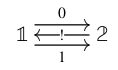
\includegraphics[width=0.15\textwidth]{1.png}
        \label{fig:1-png}
    \end{figure}
    between the categories $\mathbbm{1}$ and $\mathbbm{2}$, describe the
    corresponding natural transformations between the covariant functors
    $\Cat \to \Set$ represented by the categories $\mathbbm{1}$ and
    $\mathbbm{2}$.\\
    \linebreak
    \textit{Solution:} The functor $\mathbbm{1} \stackrel{0}{\to} \mathbbm{2}$ 
    induces a natural transformation $C(\mathbbm{2}, -) \to C(\mathbbm{1}, -)$ by
    precomposition. So for a morphism
    $f  \colon A \to B$ with $A,B \in \Cat$, we have


    \[
    \begin{tikzcd}
        C(\mathbbm{2},A) \arrow[r, "0^*"] \arrow[d, "f_*"] & C(\mathbbm{1}, A)
        \arrow[d, "f_{*}"] \\
        C(\mathbbm{2}, B) \arrow[r, "0^*"] & C(\mathbbm{1},B)
    \end{tikzcd}
    \] 
Naturality asserts that a morphism $\alpha  \colon \mathbbm{2} \to A$ mapped
as $f_* 0^{*} \alpha = f \alpha 0$ is the same as
$0^{*} f_* \alpha = f \alpha 0$, which is true.\\
\linebreak
The exact same reasoning is applied to
    \[
    \begin{tikzcd}
        C(\mathbbm{2},A) \arrow[r, "1^*"] \arrow[d, "f_*"] & C(\mathbbm{1}, A)
        \arrow[d, "f_{*}"] \\
        C(\mathbbm{2}, B) \arrow[r, "1^*"] & C(\mathbbm{1},B)
    \end{tikzcd}
    \] 
    The functor
$!  \colon \mathbbm{2} \to \mathbbm{1}$ induces a natural transformation
$C \left( \mathbbm{1}, - \right) \to C\left( \mathbbm{2},- \right) $ by
precomposition.
In this case, we have that the following square commutes for any
$f  \colon A \to B$ with $A, B \in \Cat$:

\begin{equation*}
\begin{tikzcd}
    C(\mathbbm{1}, A) \arrow[r, "!^{*}"] \arrow[d, "f_*"] & C(\mathbbm{2}, A)
    \arrow[d, "f_*"]\\
    C(\mathbbm{1},B) \arrow[r, "!^{*}"] & C(\mathbbm{2}, B)
\end{tikzcd}
\end{equation*}
which is saying that
for a morphism $\alpha  \colon \mathbbm{1} \to A$,
$f_* !^{*} \alpha = f \alpha !$ is the same as
$!^{*} f_* \alpha = f \alpha !$, which is true.


















\end{document}
